\chapter{Arcabouço Geológico da Bacia do Parnaíba}

A Bacia do Parnaíba é uma das grandes bacias intracratônicas paleozoicas do Brasil, junto com as bacias do Paraná, Solimões e Amazonas. Sua área extende-se por 600 mil $km^{2}$ na porção Norte e Nordeste do Brasil, englobando os estados do Piauí, Maranhão, Tocantins, Pará, Ceará e Bahia. Em seu depocentro, é possível observar espessuras próximas de 3.500 metros de profundidade \citep{goes_feijo_1994,vaz_bacia_2007}. Regionalmente, a Bacia do Parnaíba é bordejada por blocos cratônicos e por faixas de dobramentos brasilianas \citep{cordani_bacia_2009,de_castro_crustal_2014}. Ao norte a bacia é limitada pelas bacias sedimentares da Margem Equatorial, o Cráton São Luís e pela Faixa Gurupi. Já a oeste, pela Faixa Araguaia e pelo Cráton Amazônico. Ao leste e sul, encontra-se o Cráton São Francisco e a Província Borborema, como pode ser visto na Figura \ref{mapa_geologico}.

\begin{figure}[!ht]
\begin{center}
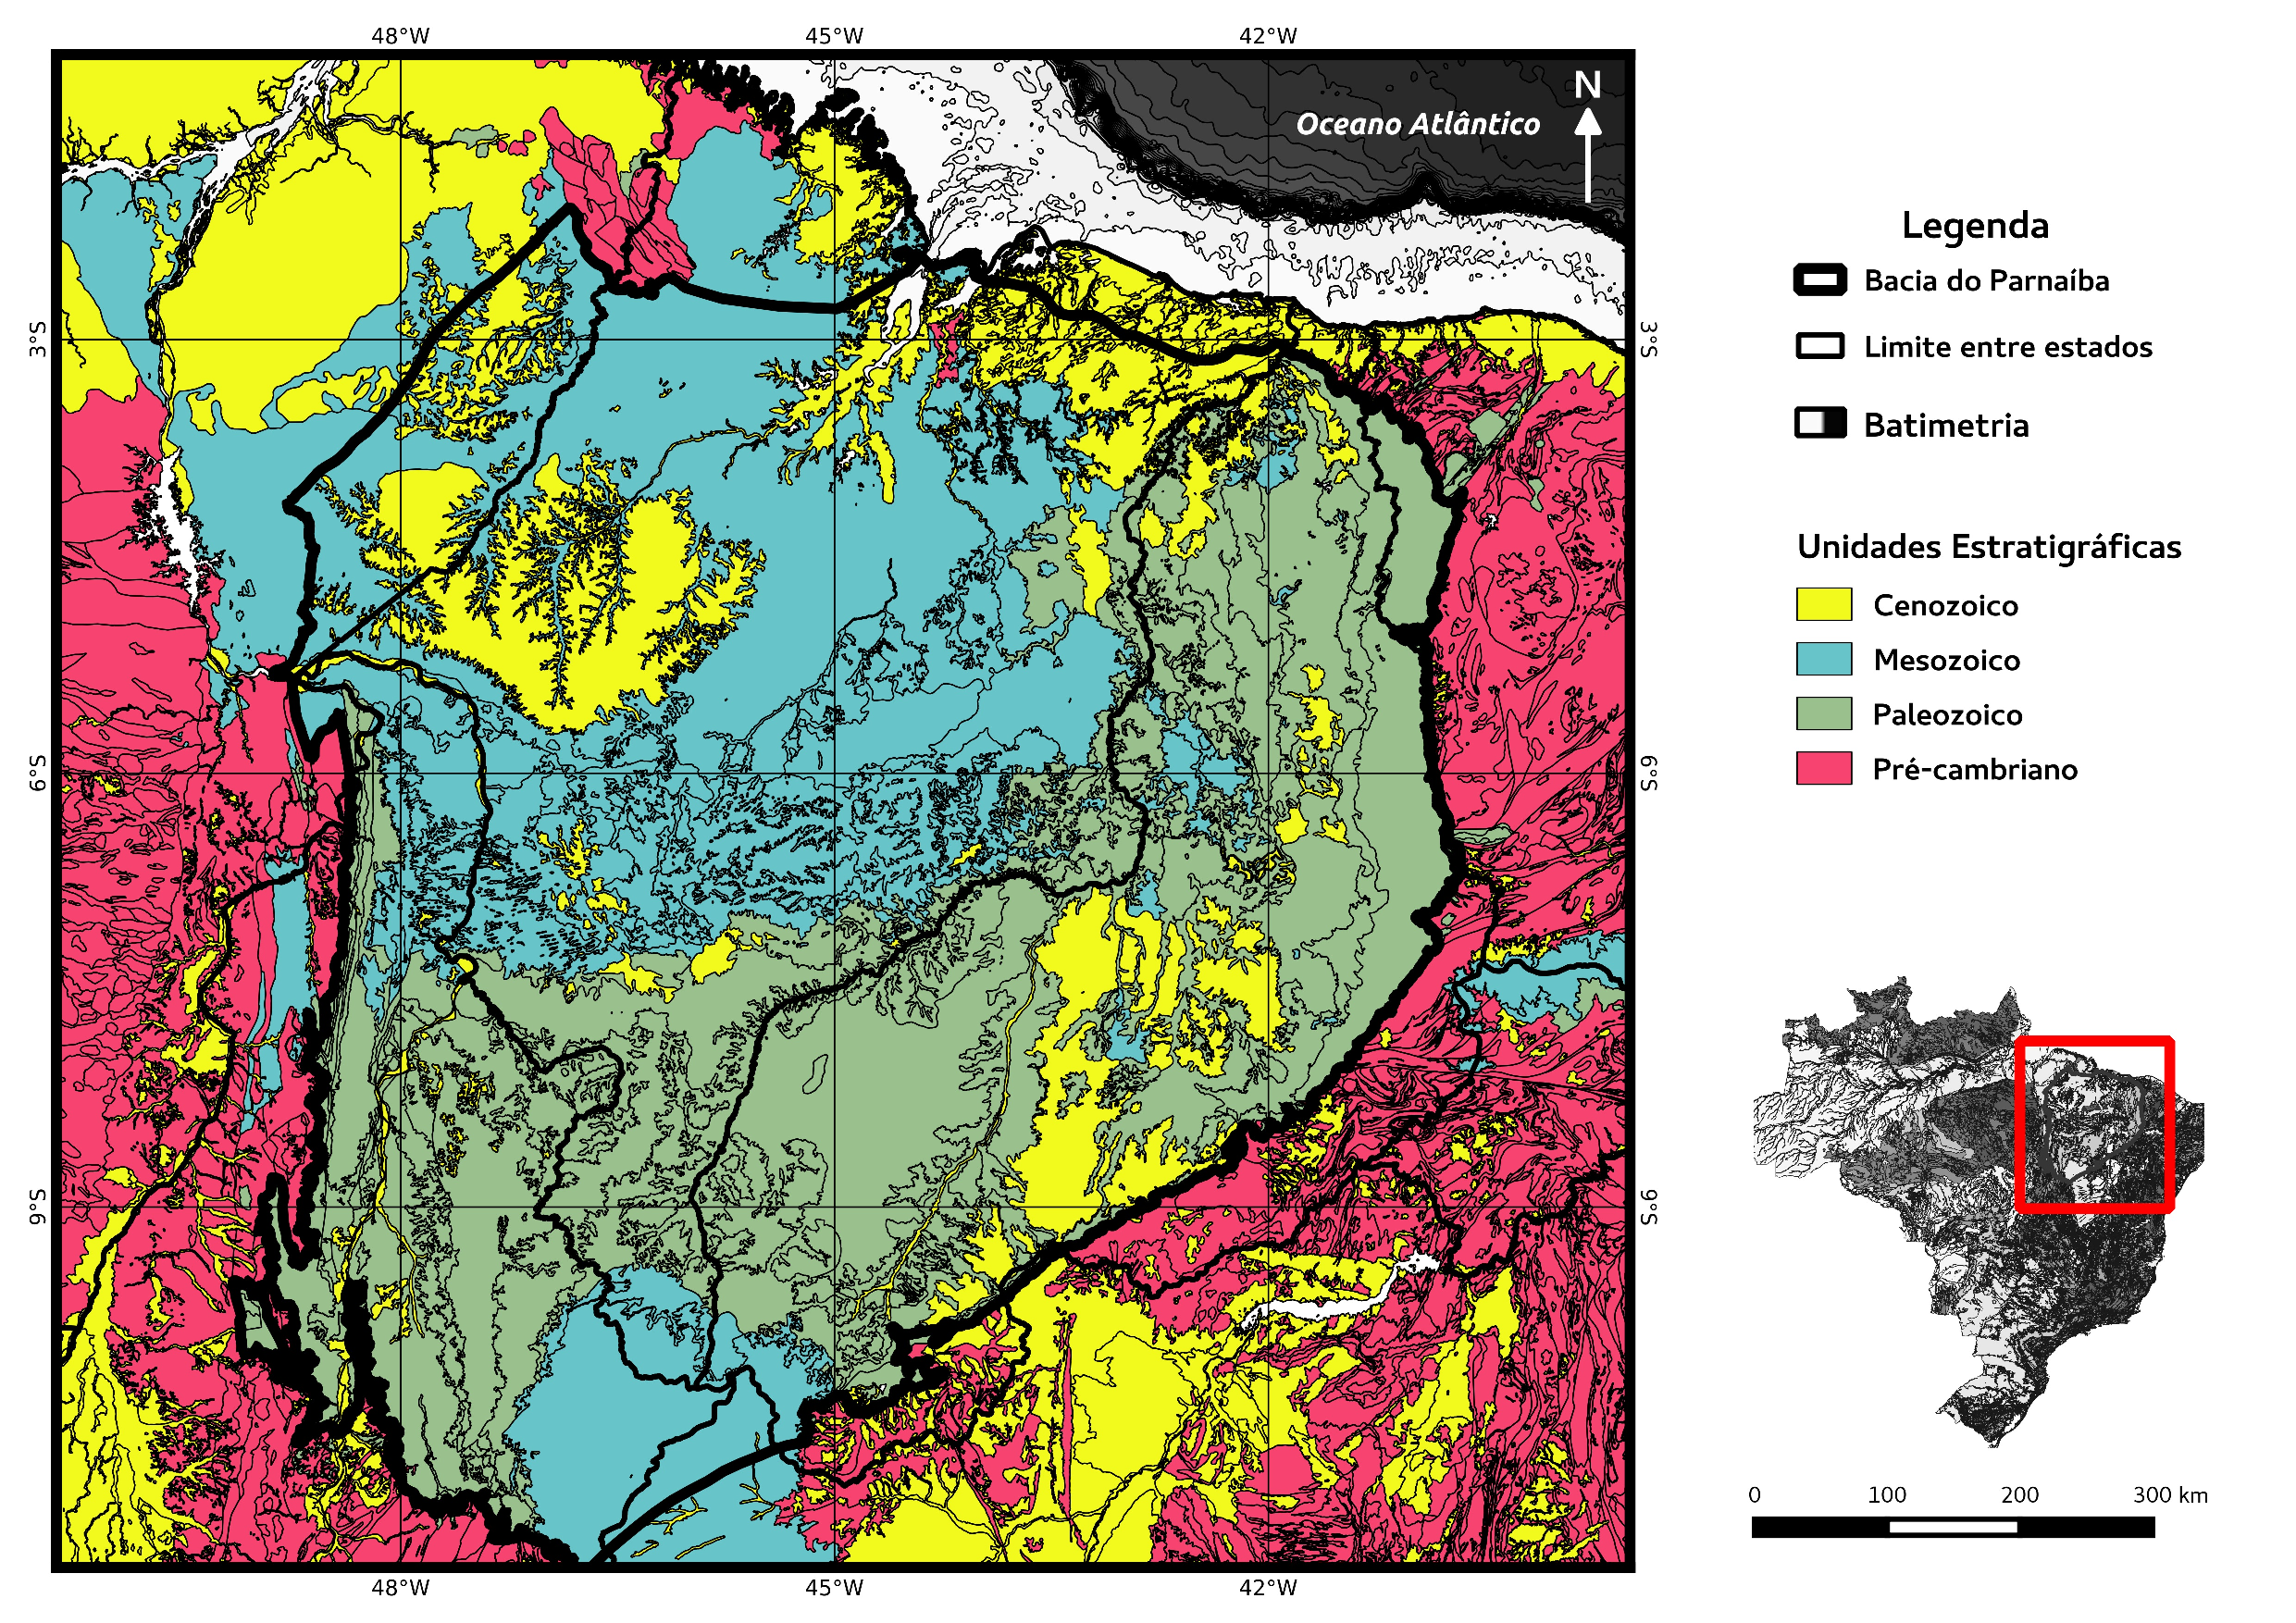
\includegraphics[width=1\textwidth]{Fig/mapa_geologico_eras.pdf}
\caption{Mapa geológico da Bacia do Parnaíba.}
\label{mapa_geologico}
\end{center}
\end{figure}

\section{Preenchimento Sedimentar}

\cite{goes_formacao_1995} aponta a dificuldade da compreensão do histórico deposicional da bacia junto com a compartimentação tectônica pré, sin e pós-ruptura do Macrocontinente Gondwana, devido a um preenchimento sedimentar com gênese, estilo tectônico e idade distinta. Com a dificuldade de relacionar todo esse registro sedimentar a uma única unidade geotectônica, sugeriu-se uma série de sub-bacias compondo uma grande provincia sedimentar, chamada Província Sedimentar do Meio-Norte. Já os trabalhos de \cite{vaz_bacia_2007,daly_brasiliano_2014,de_castro_geophysical_2016,tozer_crustal_2017} entendem que a Bacia do Parnaíba tem uma história deposicional marcada por 5 sequências tectôno-sedimentar primárias e dois pulsos magmáticos seperados por descontinuidades geológicas regionais. O preenchimento sedimentar da bacia é caracterizado pelas sequências: Riachão, Jaibaras, Parnaíba, Mearim e Grajaú. \cite{vaz_bacia_2007} mostra que as sequências Riachão e Jaibaras formam um embasamento sedimentar da Bacia do Parnaíba. Porém existe uma diversidade de interpretações sobre a formação e idades dessas sequências sedimentar, principalmente para a sequências Richão, como é visto nos trabalhos de \cite{de_castro_geophysical_2016} e \cite{tozer_crustal_2017}. As sequências inicias são interpretadas como sedimentos pretéritos oriundos de eventos de riftiamentos neoproterozóicos e cambro-ordovicianos, como mostra \cite{de_oliveira_jaibaras_2003} e \cite{de_castro_crustal_2014}. A tectônica e idade dessas sequências ainda encontra-se em discussão nas pesquisas atuais, fato que não iremos abordar neste trabalho, pois não faz parte do escopo, mas pode ser observado nos trabalhos de \cite{de_castro_crustal_2014,daly_brasiliano_2014,de_castro_geophysical_2016,tozer_crustal_2017}.

A tectono-sequência Parnaíba é relacionada a uma bacia cratônica do tipo sinéclise, denominada por \cite{goes_formacao_1995} como a Bacia do Parnaíba, propriamente dita. Essa tectono-sequência tem idade entre o Ordoviciano Tardio até o incío do Triássico e consiste de três megasequências separadas por inconformidades regionais, como pode ser visto em \cite{daly_brasiliano_2014}. Estes depósitos são caracterizados por camadas apresentando grande continuidade e espessuras regulares que se afinam progressivamente em direção às bordas da bacia, um comportamento característico do estilo de bacia do tipo sag. Os tipos de sedimentos associados a essa fase são marinhos rasos, fluvio-lacustre e siliciclásticos terrestres. 

\cite{vaz_bacia_2007} mostra que a tectono-sequência Mearim, ou Jurássica, é composta apenas pela Formação Pastos Bons, que corresponde a depósitos lacustrinos com contribuição fluvial, em clima semi-árido a árido. A sequência é balizada na base e no topo por episódios magmáticos e é restrita apenas ao centro da bacia \citep{tozer_crustal_2017}. Já a tectono-sequência Grajaú (Cretácea) é caracterizada por depósitos marinhos rasos, lacustres e flúvio-deltaicos, cuja deposição seria reflexo da abertura do Oceano Atlântico \citep{vaz_bacia_2007}. Em afloramento, essa seqüência ocorre principalmente na porção noroeste-norte da bacia e sobrepõe-se discordantemente sobre as rochas das seqüências mais antigas. É importante frisar que o depocentro se deslocou durante a fase deposicional da bacia, com uma forte tendência para oeste, como mostra \cite{tozer_crustal_2017} através de dados de backstripping. 

\section{Magmatismo}

A intensa atividade ígnea em que foram palcos as bacias do Parnaíba, Paraná, Amazonas e Solimões teve início com a abertura da Margem Equatorial durante a separação entre os continentes sul-americano e africano. Segundo \cite{vaz_bacia_2007} a Bacia do Parnaíba acomodou rochas ígneas intrusivas, diques e soleiras, e extrusivas de composição básica, as quais foram divididas em duas unidades: Formação Mosquito e Formação Sardinha. Essas formações são correlacionadas às rochas originadas a partir do rifteamento do supercontinente Pangea e da abertura do Oceano Atlântico, respectivamente. As idades isotópicas calculadas por \cite{merle_40ar_39ar_2011} apontam que a Formação Mosquito pertence à Província Magmática do Atlântico Central, já a formação Sardinha seria associada à Província Magmática Paraná-Etendeka.

Eventos precursores à desagregação do Gondwana Oeste propiciaram o abatimento da região central da bacia, com a formação de um sistema de riftes interiores, preenchidos pelos sedimentos das formações Pastos Bons e Corda associados ao alojamento das rochas básicas das formações Mosquito e Sardinha. A implantação desses riftes ocorreu, principalmente, sobre área da Estrutura de Xambioá, como mostra \cite{mocitaiba_cartografia_2017}. As estruturas grabenformes geradas permitiram o alojamento desses eventos ígneos mesozoicos. Em subsuperfície, os diques da Formação Sardinha e as soleiras da Formação Mosquito estão presentes em maior quantidade na tectono-sequência paleozoicas \citep{vaz_bacia_2007}.

\section{Tectônica}

A bacia do Parnaíba é circundada por inúmeras massas cratônicas arqueanas e por cinturões de dobramentos proterozoicos, como pode ser visto na Figura \ref{mapa_geologico}. Dois desses principais blocos formaram duas grandes massas continentais (São Franciso-Congo e São Luís-West Africa) que existiram antes da abertura do oceano Atlântico no mesozoico, e estavam envolvendo o bloco da Parnaíba, provável massa cratônica coberta pela bacia homônima. A existência desse bloco ocultado pela cobertura sedimentar foi postulada por inúmeras trabalhos nos ramos da geofísica, petrofísica, tectônica e geocronologia \citep{de_brito_neves_influence_1984, cordani_bacia_2009,fuck_rodinia_2008,de_castro_crustal_2014}. Análises de dados magnéticos e gravimétricos recentemente subdividiram esse bloco Parnaíba em pequenos fragmentos, denominados Parnaíba Norte, Parnaíba Sul e Teresina. Estes caracterizados pelas mudanças marcantes nas propriedades magnéticas e pelas variações de até 3.5 km na espessura crustal \citep{de_castro_crustal_2014}. 

No passado, estudos geofísicos da Bacia do Parnaíba delinearam uma grande quantidade de estruturas grabenformes abaixo da cobertura sedimentar, como mostra \cite{de_brito_neves_influence_1984,cordani_bacia_2009}. Essas estruturas interpretadas foram utilizadas como suporte para modelos de subsidência termo-mecânicos, como o clássico modelo de \cite{mckenzie_remarks_1978}. Um refinamento mais recente deste conjunto de modelos foi proposto por \cite{de_castro_crustal_2014}, pela análise de anomalias gravimétricas e magnéticas. Os autores identificaram dois conjuntos de trends lineares no embasamento, o qual foram interpretados como dois estágios de riftiamento, um relacionado ao fim da orogenia Brasiliana e o outro precedendo a fase deposicional principal da bacia no Cambro-Ordoviciano. 
Em um grande perfil de reflexão sísmica profunda \cite{daly_brasiliano_2014} não encontrou evidência de uma fase de riftiamento neoproterozóica postulada previamente, e notou uma inconformidade subplanar cortando todos os blocos crustais interpretados no perfil, Borborema, Parnaíba e Amazônico. Segundo os autores, os limites principais e as estruturas do embasamento não teriam uma grande influência na formação da bacia e propõem que uma subsidência termal se tornaria um provável mecanismo para a formação e evolução da bacia do Parnaíba.

A viabilidade de um modelo de riftiamento para a bacia foi investigada exaustivamente por \cite{tozer_crustal_2017} através dos estudos das anomalias Bougher desenvolvidas em cima do mesmo perfil sísmico de \cite{daly_brasiliano_2014}, backstripping dos dados de poços disponíveis e da modelagem sísmica de uma rede densa de receptores no centro da transecta. O estudo demonstrou que o modelo de riftiamento não é capaz de explicar as estruturas crustais inferidas, assim como a história de subsidência dessa bacia. Devido a grande quantidade de intrusões magmáticas na bacia, os autores postularam existência de uma grande corpo máfico de 12-20 km de espessura na crosta inferior que serviria como um carga que causaria uma subsidência flexural. Através da relaxão do esforço viscoelástico essa carga poderia explicar a longa história de subsidência observada nos registros de poços. No entanto, os autores não restringem os limites dessa carga em profundidade e ainda não existem evidências geológicas de um magmatismo extensivo no início da bacia, prova cabal para poder afirmar esse corpo magmático na crosta inferior.